\title{Einleitung}
\chapter{Was ist yocto}




%
%
%Anschließend einen \textbf{Projektnamen} vergeben und einen \textbf{Leere/Hallo-World} \glqq Projekt-Typ \grqq wählen. Als \textbf{\glqq Toolchains \grqq} \textbf{\glqq Cross GCC \grqq} wählen. 
%
%\begin{figure}[h!]
%\centering
%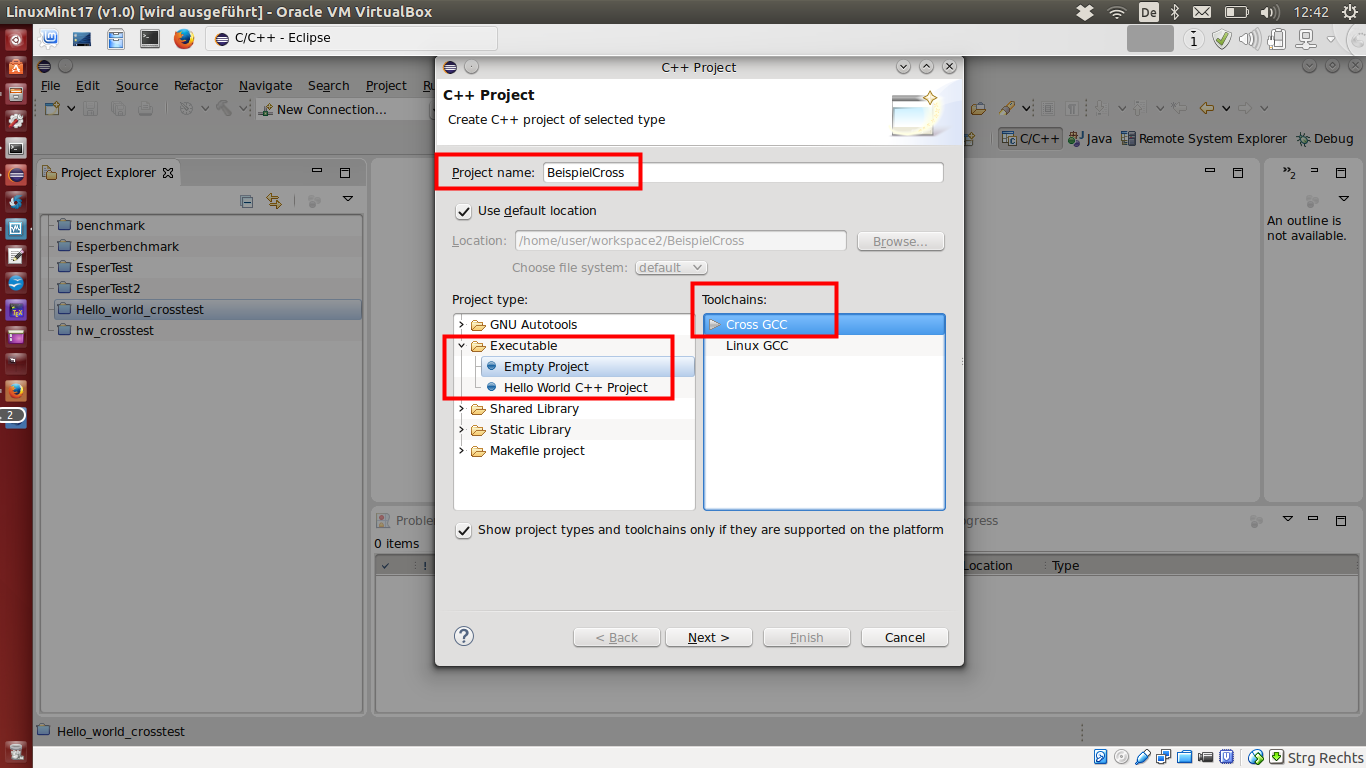
\includegraphics[width=0.9\linewidth]{./pictures/neu2.png}
%\caption[neu2]{}
%\label{fig:neu2}
%\end{figure} 
%\vspace{10cm}
%
%So lange auf \glqq \textbf{weiter/next} \grqq, bis das nachfolgende Fenster erscheint. In diesem überprüfen ob als \glqq \textbf{Cross Compiler Prefix} \grqq \glqq \textbf{arm-linux-gnueabihf-} \grqq
%eingetragen ist. (Dies sollte die Voreinstellung sein).\\
%\begin{figure}[h!]
%\centering
%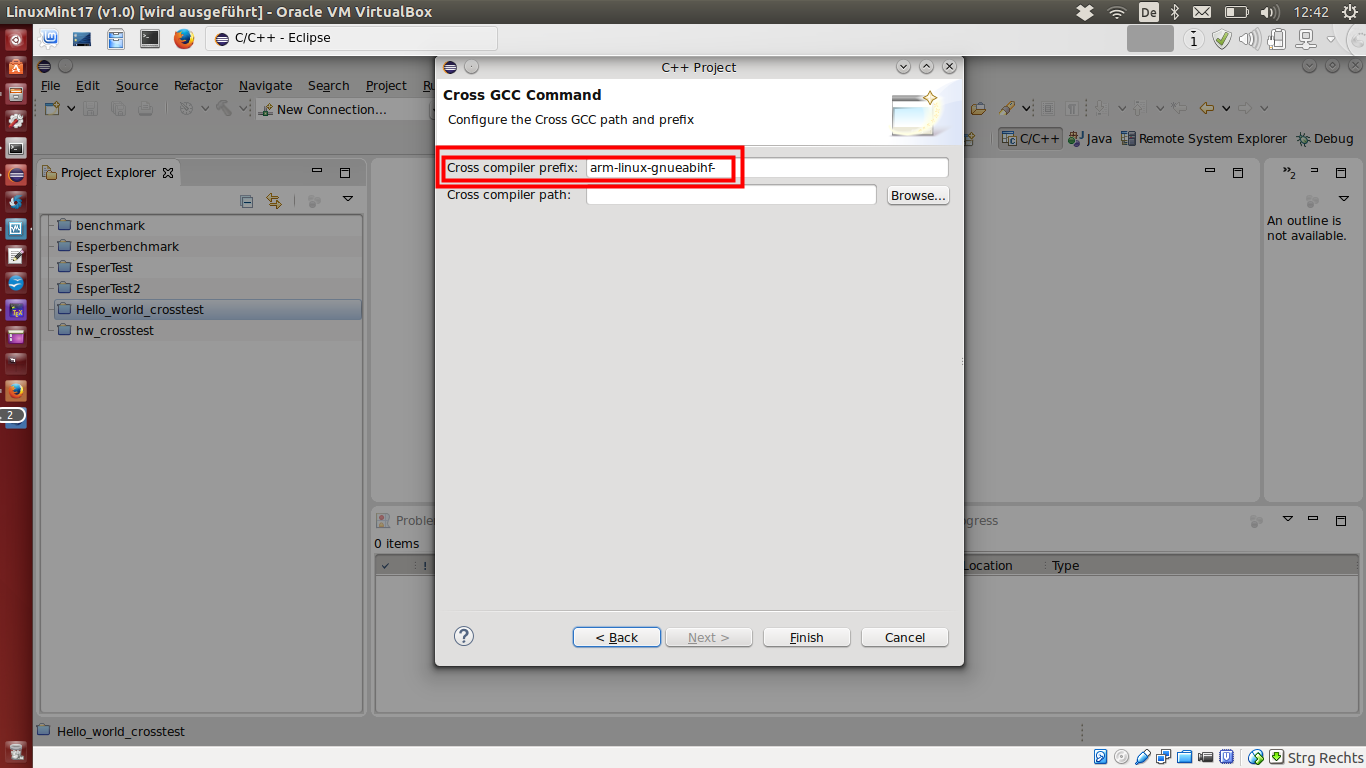
\includegraphics[width=0.9\linewidth]{./pictures/neu3.png}
%\caption[neu3]{}
%\label{fig:neu3}
%\end{figure} 
%
%Anschließend sollte das Projekt verfügbar sein:\\
%\begin{figure}[h!]
%\centering
%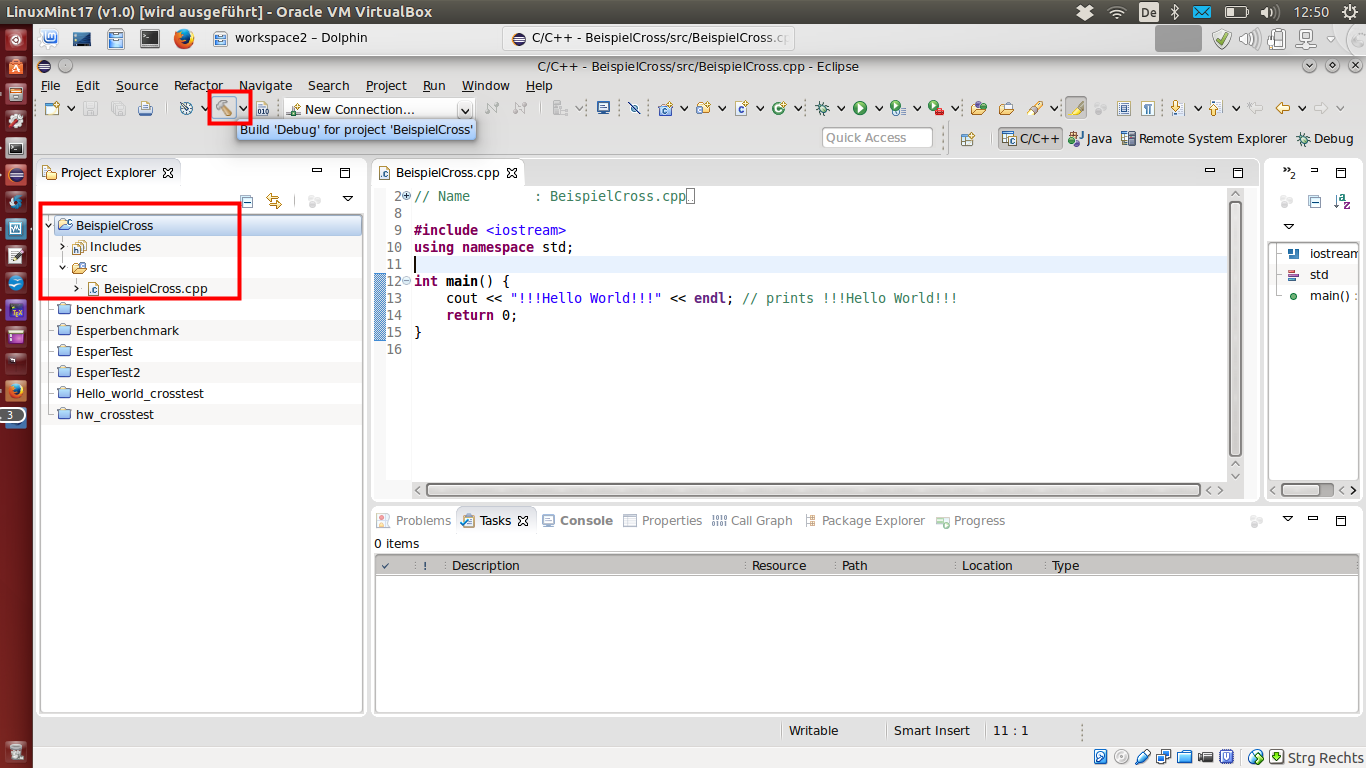
\includegraphics[width=0.9\linewidth]{./pictures/neu4.png}
%\caption[neu4]{}
%\label{fig:neu4}
%\end{figure} 
%\newline
%Das Projekt muss nun \glqq gebaut \grqq und ggf. einmal ausgeführt werden. So wird der Order \glqq Debugg \grqq sowie die ausführbaren Dateien erzeugt. 
%
%
%\begin{figure}[h!]
%\centering
%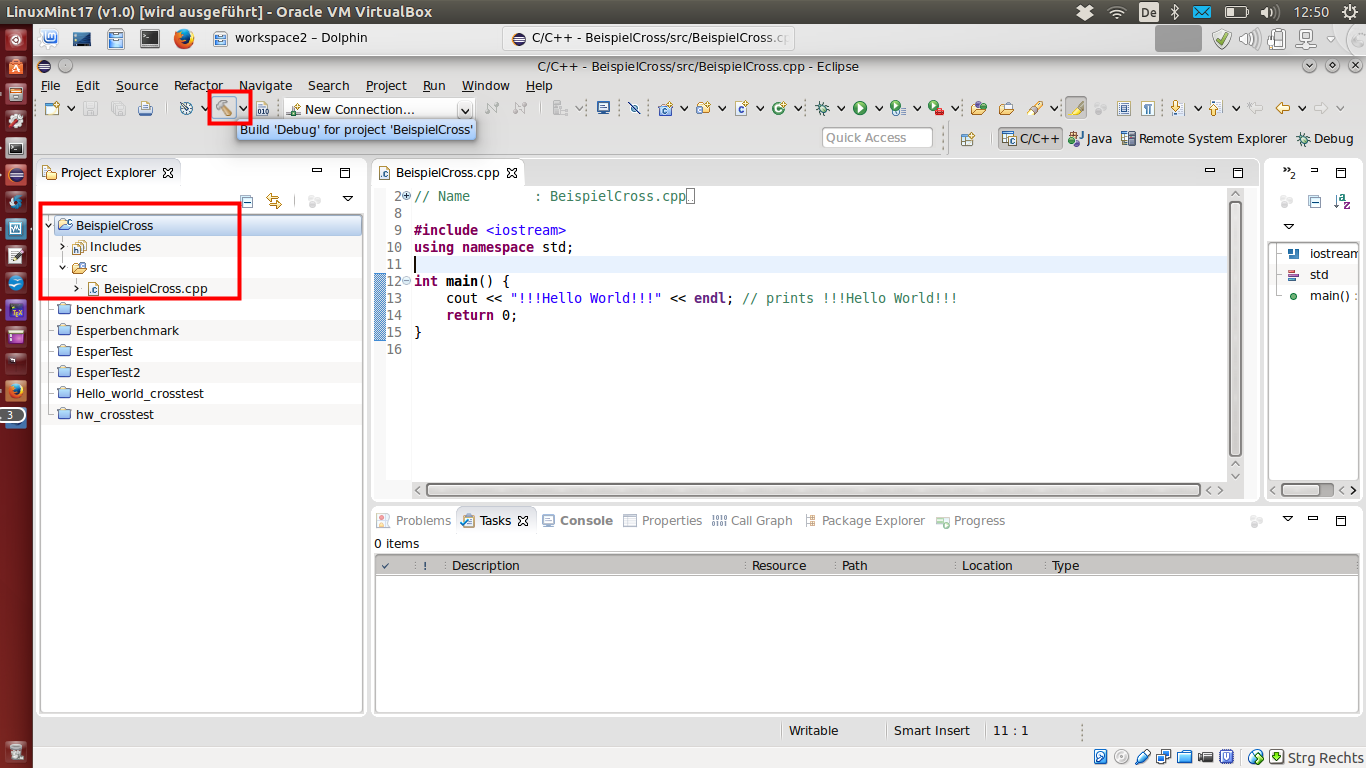
\includegraphics[width=0.9\linewidth]{./pictures/neu4.png}
%\caption[neu4]{}
%\label{fig:neu4}
%\end{figure} 
%\vspace{1cm}
%
%\chapter{Netzwerkverbindung einrichten}
%Um das Target als Ziel zum \glqq  Remote Compile \grqq und \glqq  Remote Debugg \grqq auswählen zu können, muss dieses und seiner IP adresse angelegt werden.
%
%Hierzu den \glqq \textbf{ Reote Explorer } \grqq Modus öffnen. \glqq \textbf{Rechtsklick auf eins derbereits angeegtenGeräte } \grqq --> \glqq \textbf{Properties}\grqq
%\begin{figure}[h!]
%\centering
%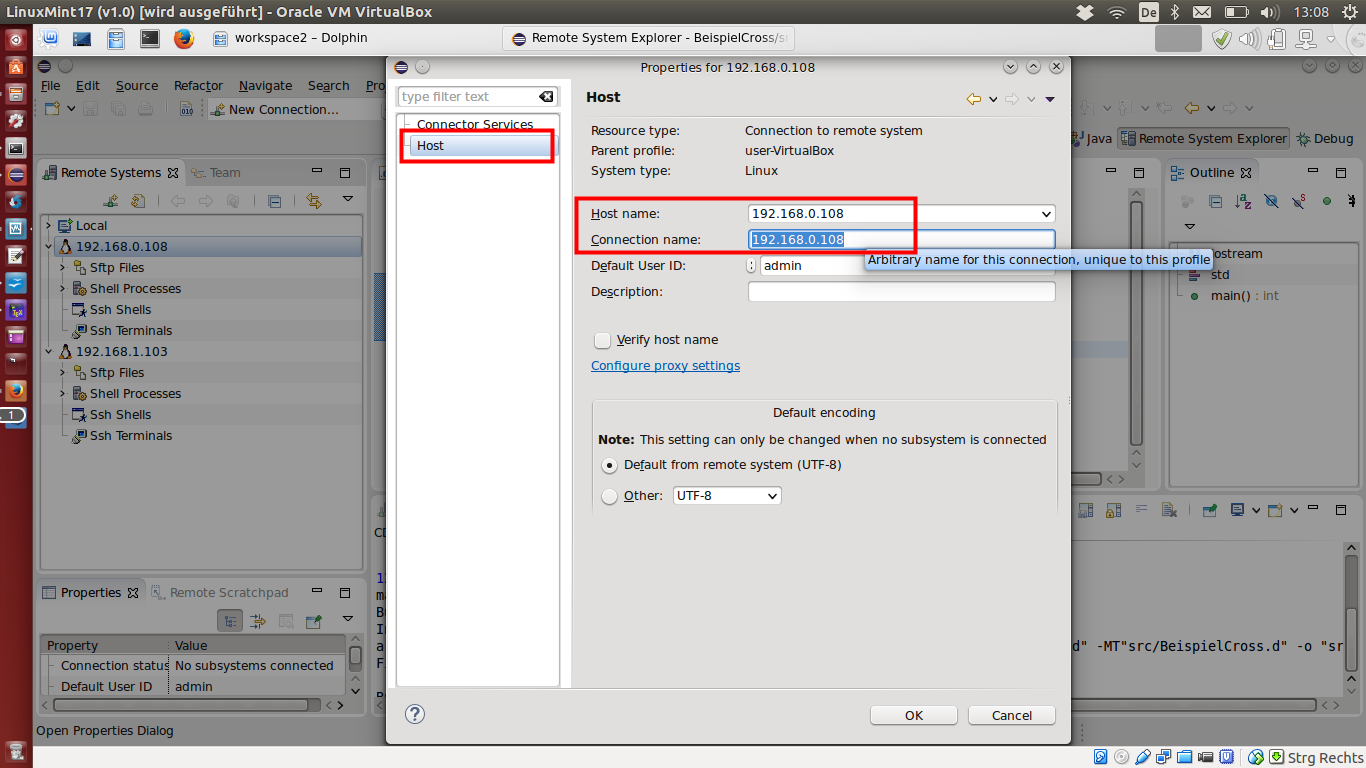
\includegraphics[width=0.8\linewidth]{./pictures/netz1.png}
%\caption[netz1]{}
%\label{fig:netz1}
%\end{figure} 
%
%Anschließend \glqq \textbf{Host} \grqq auswählen und dort die \textbf{IP-Adresse anpassen}
%\begin{figure}[h!]
%\centering
%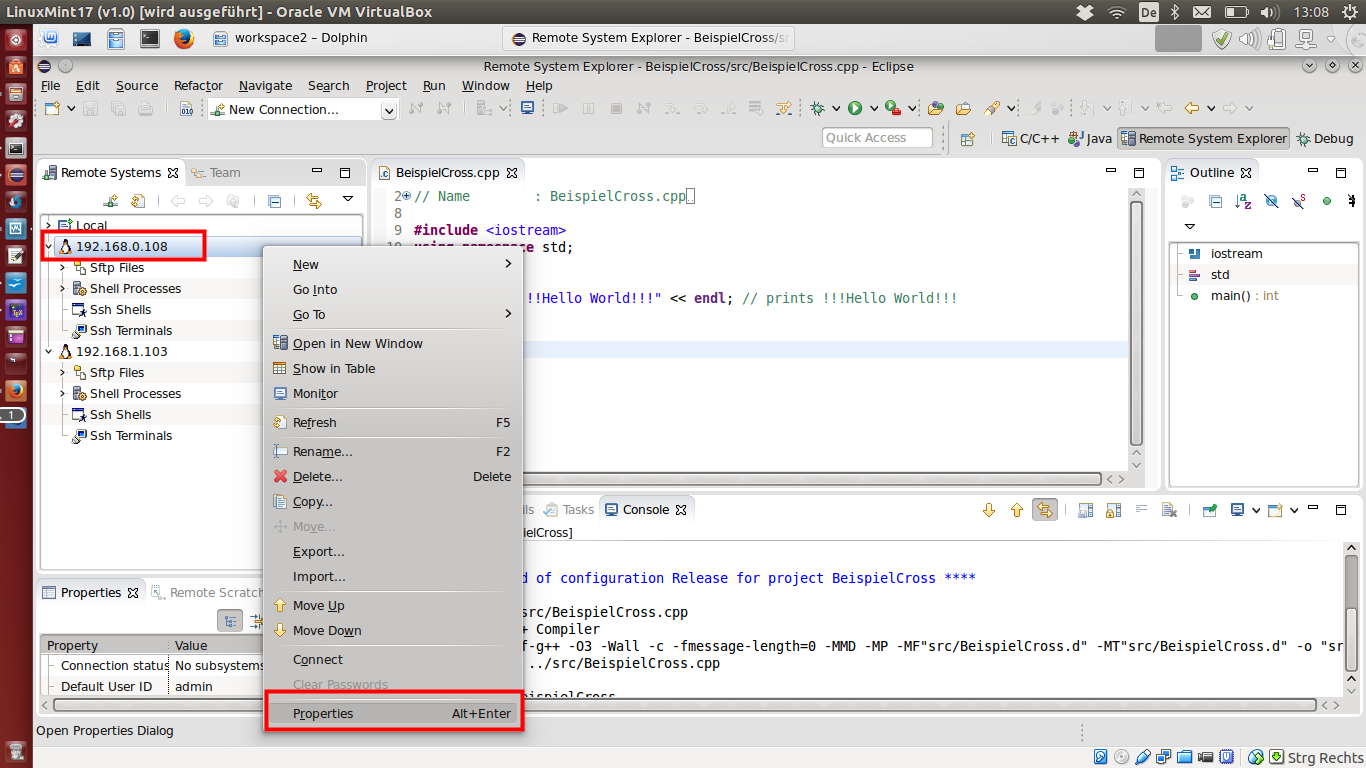
\includegraphics[width=0.8\linewidth]{./pictures/netz2.png}
%\caption[netz2]{}
%\label{fig:netz2}
%\end{figure}
%
%\chapter{Cross Compile und Remote Exekution}
%Zum Projekt ausführen: \glqq \textbf{Rechtsklick auf das Projekt } \grqq --> \glqq \textbf{Run As} \grqq --> \glqq \textbf{ Run Configurations ... } \grqq
%\begin{figure}[h!]
%\centering
%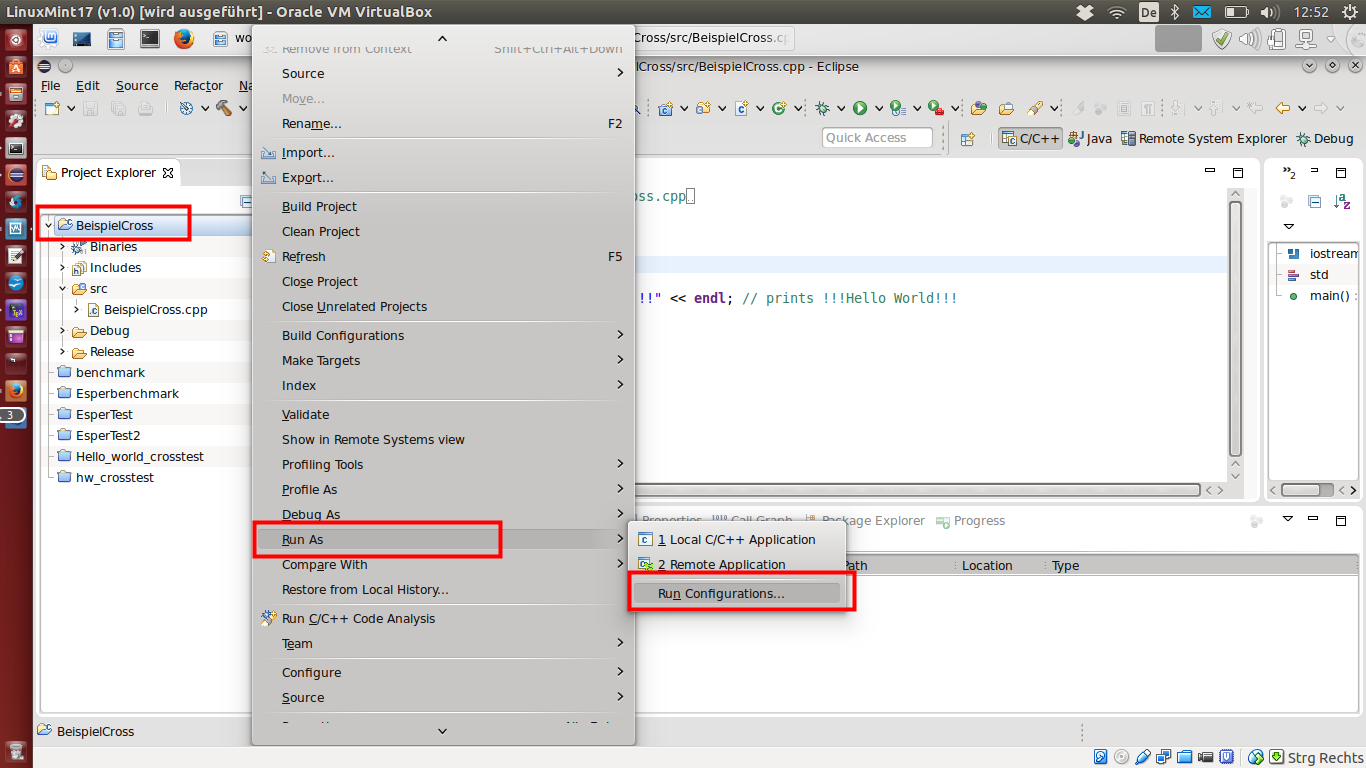
\includegraphics[width=0.9\linewidth]{./pictures/run1.png}
%\caption[run1]{}
%\label{fig:run1}
%\end{figure}
%\newline
%Es öffnet sich ein neues Fenster:
%\begin{figure}[h!]
%\centering
%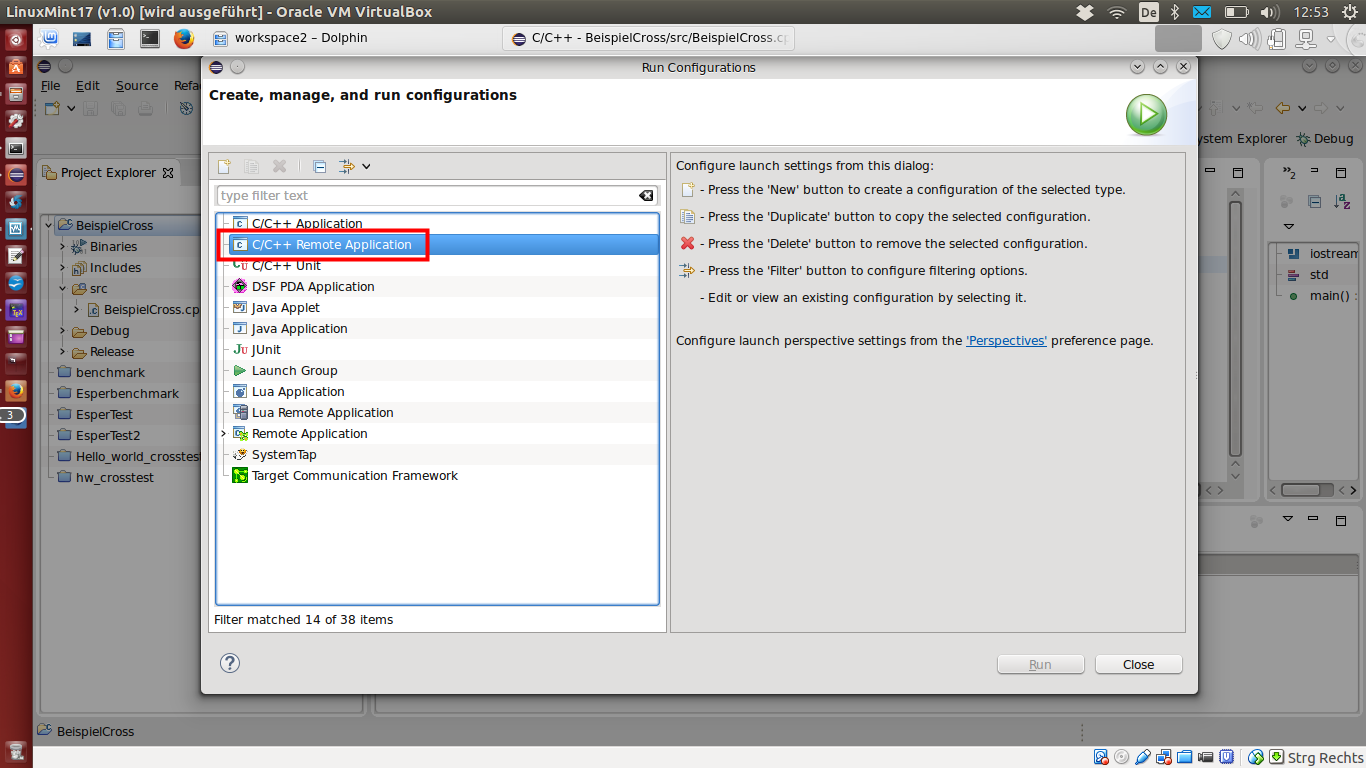
\includegraphics[width=0.9\linewidth]{./pictures/run2.png}
%\caption[run2]{}
%\label{fig:run2}
%\end{figure} 
%\newline
%\\
%In diesem einen \glqq \textbf{Doppelklick} \grqq auf \glqq \textbf{Remote Applikation} \grqq. Es wird eine neuer Eintrag für das aktuelle Projekt angelegt.
%\begin{figure}[h!]
%\centering
%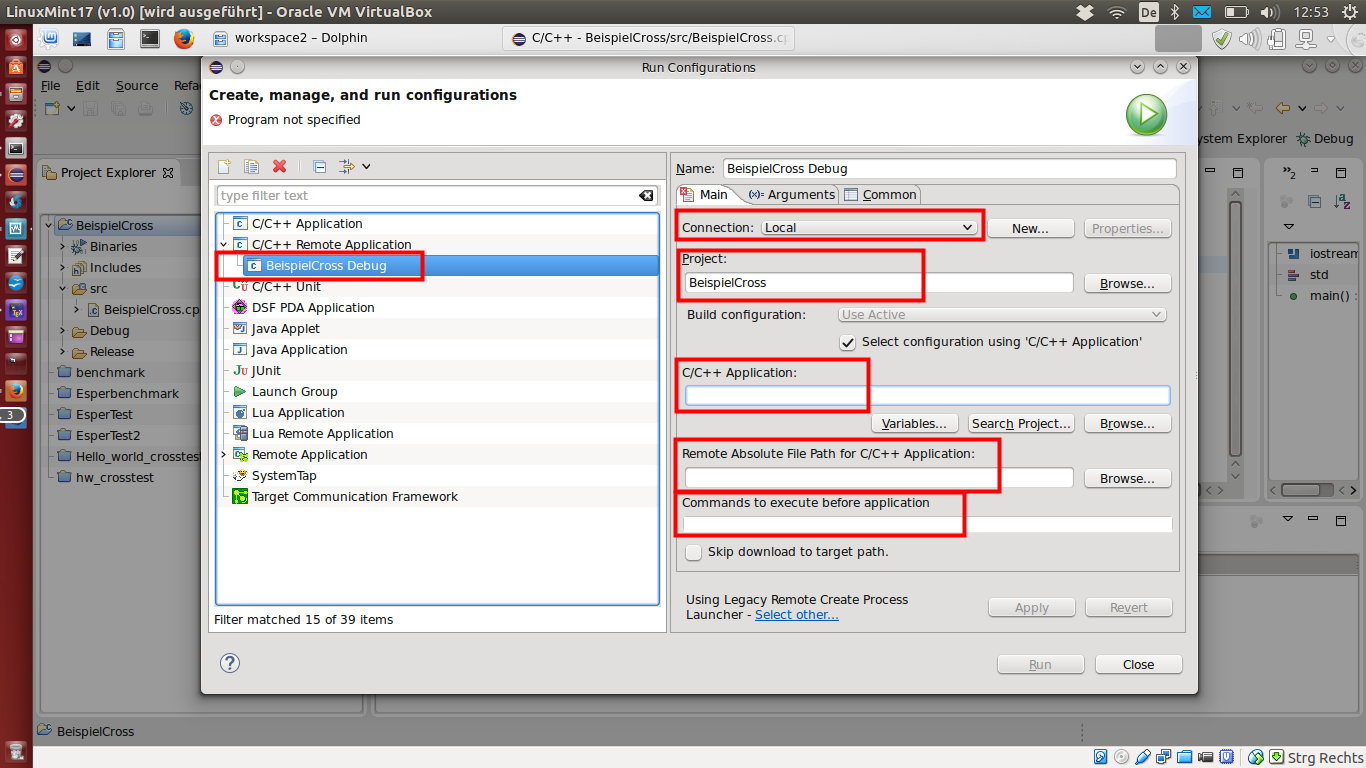
\includegraphics[width=0.9\linewidth]{./pictures/run3.png}
%\caption[run3]{}
%\label{fig:run3}
%\end{figure} 
%\newline
%
%Diesen Eintrag auswählen und die rot markierten Felder konfigurieren.\\
%Im Feld \glqq \textbf{Application} \grqq das aktuelle Programm angeben. Dieses liegt im aktuellen Projektverzeichnis im \glqq \textbf{Debug Ordner} \grqq (Ordner nicht vorhanden: siehe \glqq Fehlerbehandlung P1 \grqq). 
%\begin{figure}[h!]
%\centering
%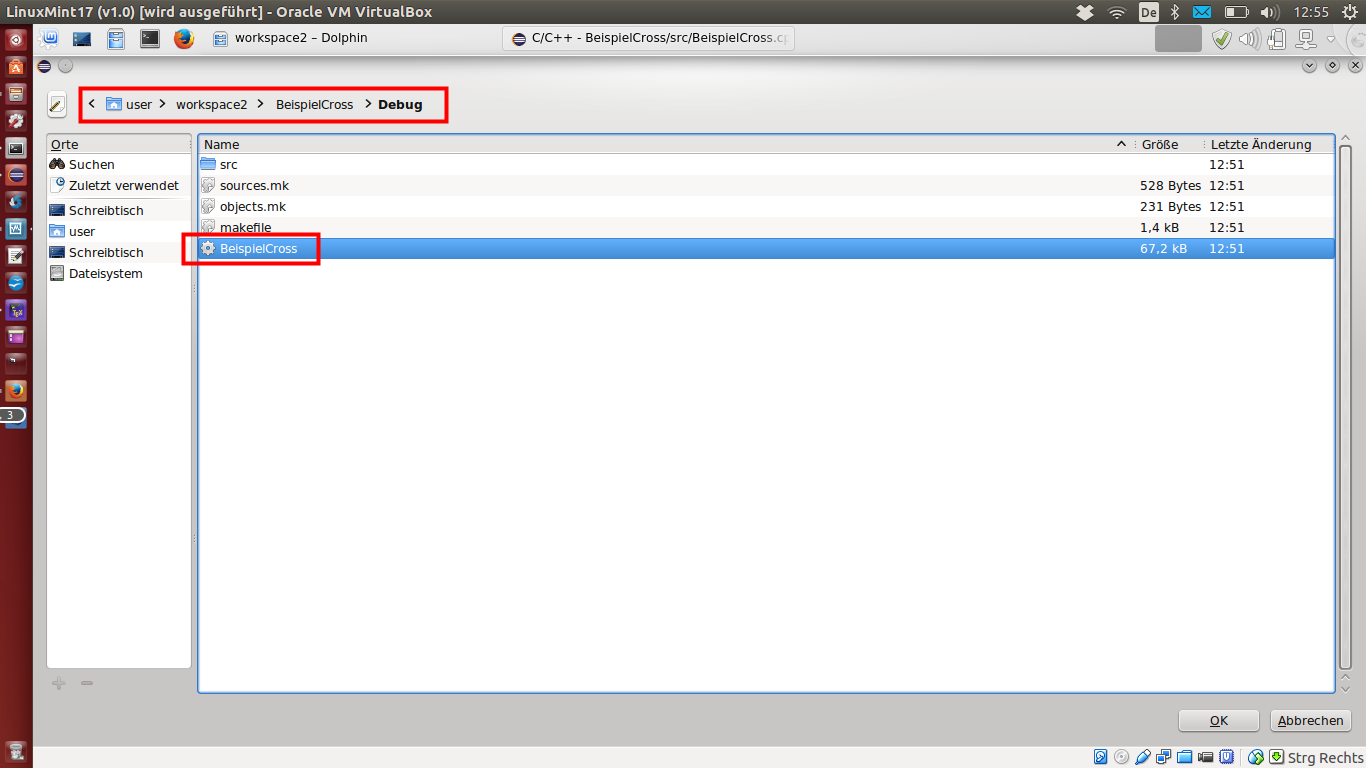
\includegraphics[width=0.9\linewidth]{./pictures/run5.png}
%\caption[run5]{}
%\label{fig:run5}
%\end{figure}
%\newline
%\vspace{3cm}
%
%Die ausgefüllte Konfiguration könnte wie folgt aussehen: 
%\begin{figure}[h!]
%\centering
%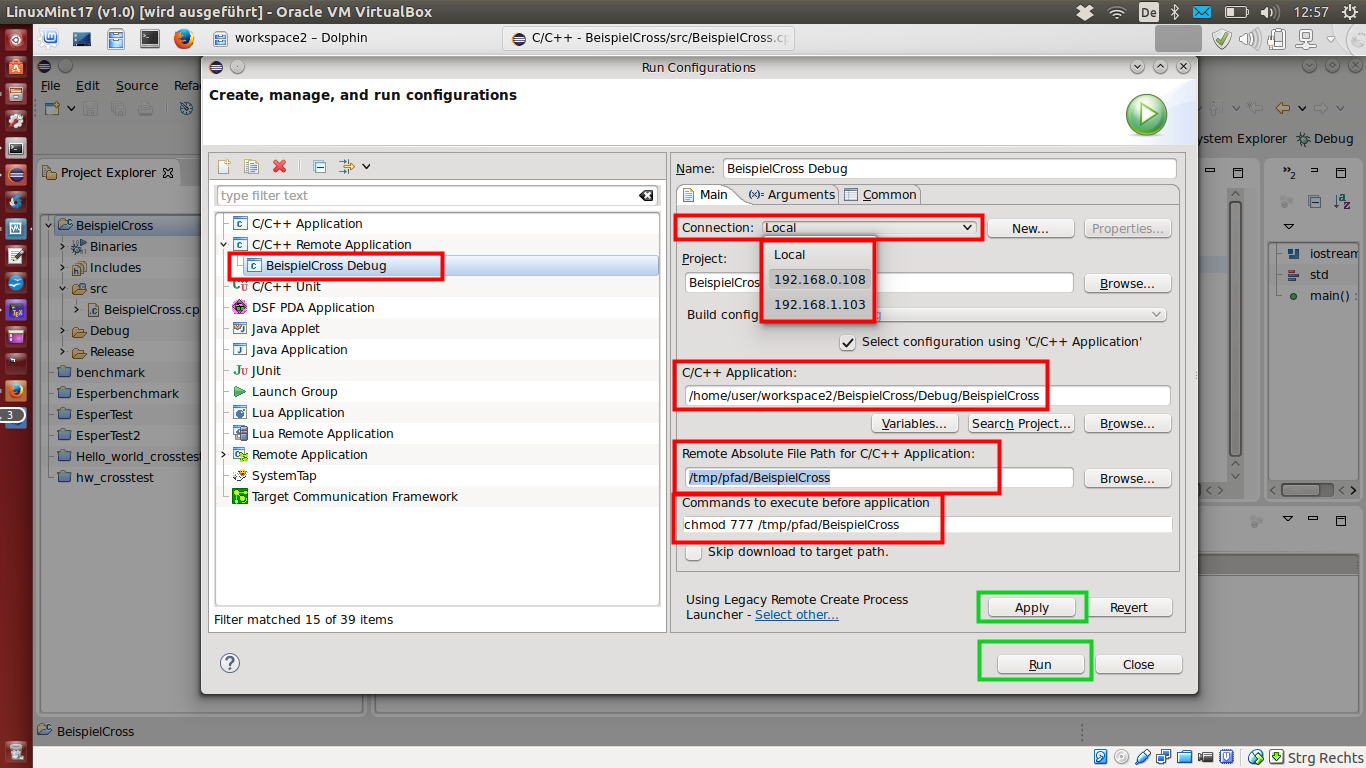
\includegraphics[width=0.9\linewidth]{./pictures/run4.png}
%\caption[run4]{}
%\label{fig:run4}
%\end{figure} 
%\newline
%
%\textbf{Wichtige Felder}: 
%\begin{description}
%\item [Connection :] Über das \glqq \textbf{Dropp Down} \grqq die \glqq \textbf{IP des Targets} \grqq auswählen. (Target nicht vorhanden: Siehe \grqq Fehlerbehandlung P2; \grqq \textbf{Connection ausgegraut} oder lässt sich nicht auswählen: Siehe \glqq Fehlerbehandlung P3 \grqq)
%\item [C/C++ Application:] 
%\item [Remote Abselute File Path for C/C++ Application:] Der Dateipfad auf dem Target. \textbf{WICHTIG:}
%\begin{itemize}
%\item \textbf{Der Dateipfad (Oderner) muss auf dem Target vorhanden sein}.
%\item Es \textbf{muss der Dateiname angegeben sein}.
%\end{itemize}
%
%\item [Commands to process before Application:] Ein Kommando das Ausgeführt werden soll, bevor die die Datei ausgeführt wird 
%\item [Using ...:] Wichtig: Hier muss \glqq \textbf{Legacy Remote Create Process Launcher} \grqq stehen. Sonst siehe \grqq Fehlerbehandlung P3; \grqq.
%\end{description}
%\vspace{4cm}
%Anschließend kann das Programm über die Button \glqq \textbf{Applay} \grqq und \glqq \textbf{Run} \grqq (grün markiert)auf dem Target ausgeführt werden. Hierzu wird das Projekt auf dem lokalen Gerät kompiliert, eine ausführbare Datei erzeugt und diese auf das Taget übertragen. Diese übertragene, ausführbare Datei wird auf dem Target ausgeführt. Sollte es zu Fehlern kommen: Siehe \grqq Fehlerbehandlung P2 \grqq und  \grqq Fehlerbehandlung P4 \grqq.\\
%GGf. erscheint ein Fenster, in welchem die Login-Daten eines Users des Target eingegeben werden müssen.
%\begin{figure}[h!]
%\centering
%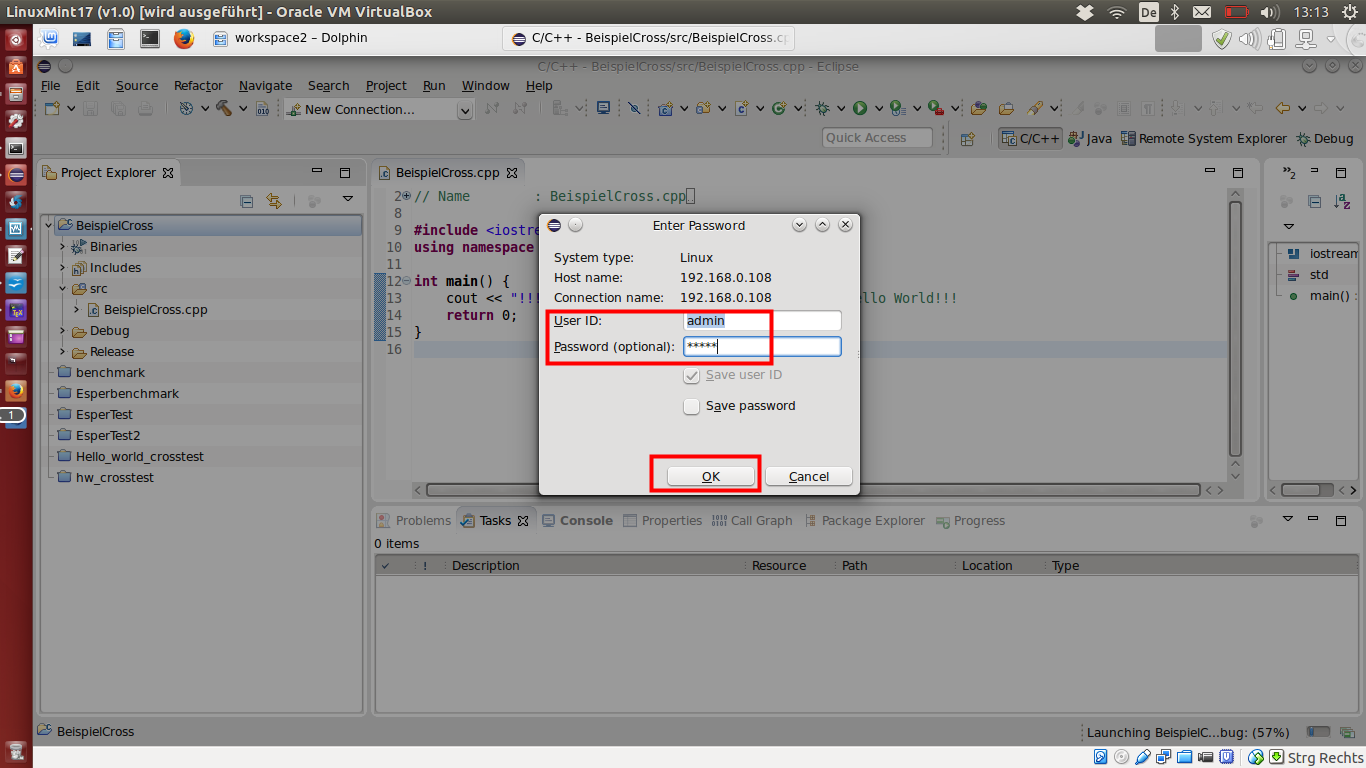
\includegraphics[width=0.9\linewidth]{./pictures/connect.png}
%\caption[connect]{}
%\label{fig:connect}
%\end{figure}
% \vspace{1cm}
%
%
%\section{Bekannte Fehler}
%\begin{description}
%\item [P1:] Ist der \glqq \textbf{ Debugg Ordner} \grqq (Abbildung \ref{fig:run5}) nicht vorhanden, wurde das Projekt zuvor nicht über den \glqq \textbf{Hammer} \grqq gebaut (Kompiliert) oder es sind dabei Fehler aufgetreten. 
%\item [P2:] Die \textbf{aktuelle Target IP } wurde unter \glqq \textbf{Remote System Explorer} \grqq nicht konfiguriert: Siehe Kapitel \glqq  \textbf{Netzwerkverbindung einrichten} \grqq. Oder die Geräte befinden sich nicht im \textbf{selben \glqq Subnetzwerk \grqq}
%\item [P3:] der \glqq \textbf{Remote Create Process Launcher} \grqq kann über den \glqq \textbf{Select other ...} \grqq Link geändert werden.
%\end{description}
%\begin{figure}[h!]
%\centering
%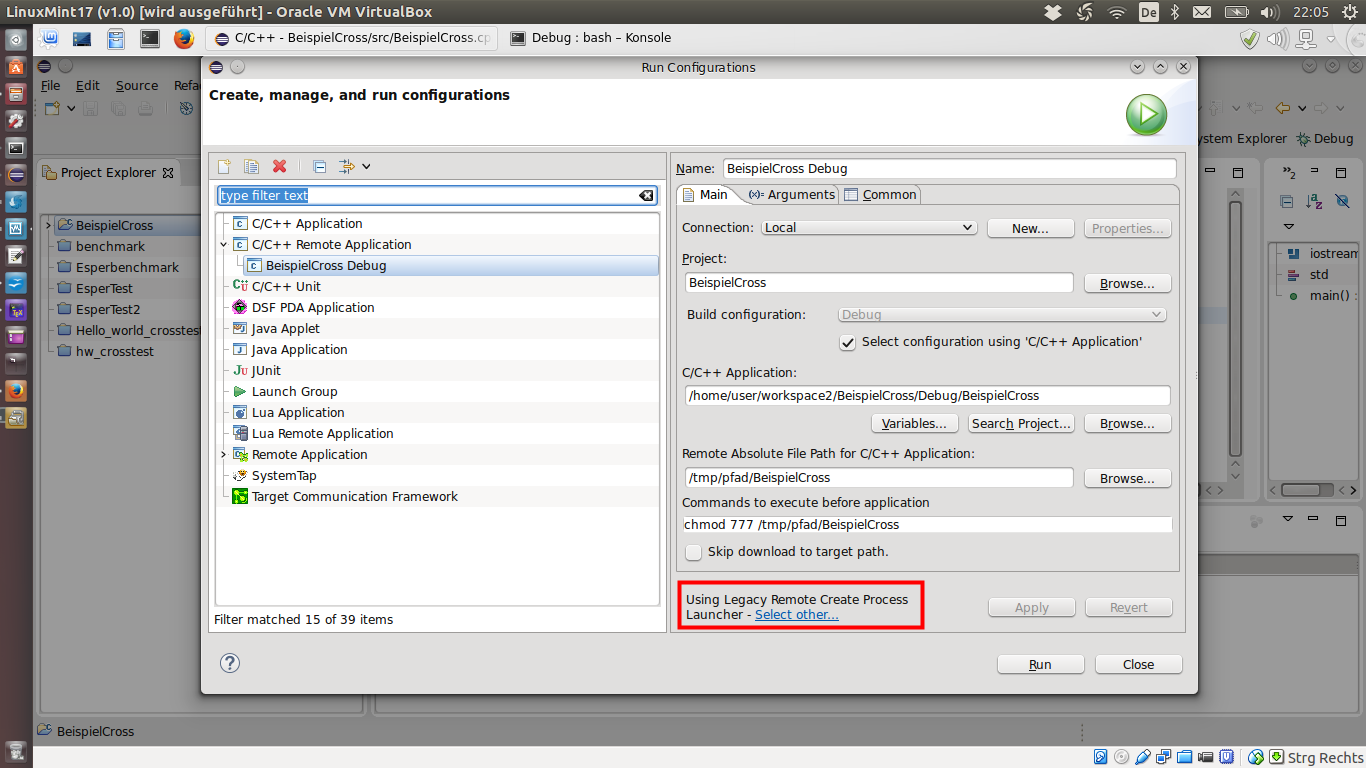
\includegraphics[width=0.9\linewidth]{./pictures/runf1.png}
%\caption[runf1]{}
%\label{fig:runf1}
%\end{figure} 
%\vspace{3cm}
%In dem nachfolgenden Fenster den \glqq \textbf{Legacy Remote Create Process Launcher} \grqq auswählen. Hierzu muss der \glqq  \textbf{Hacken} \grqq bei \glqq \textbf{Using configuration specific setings} \grqq gesetzt sein 
%\begin{figure}[h!]
%\centering
%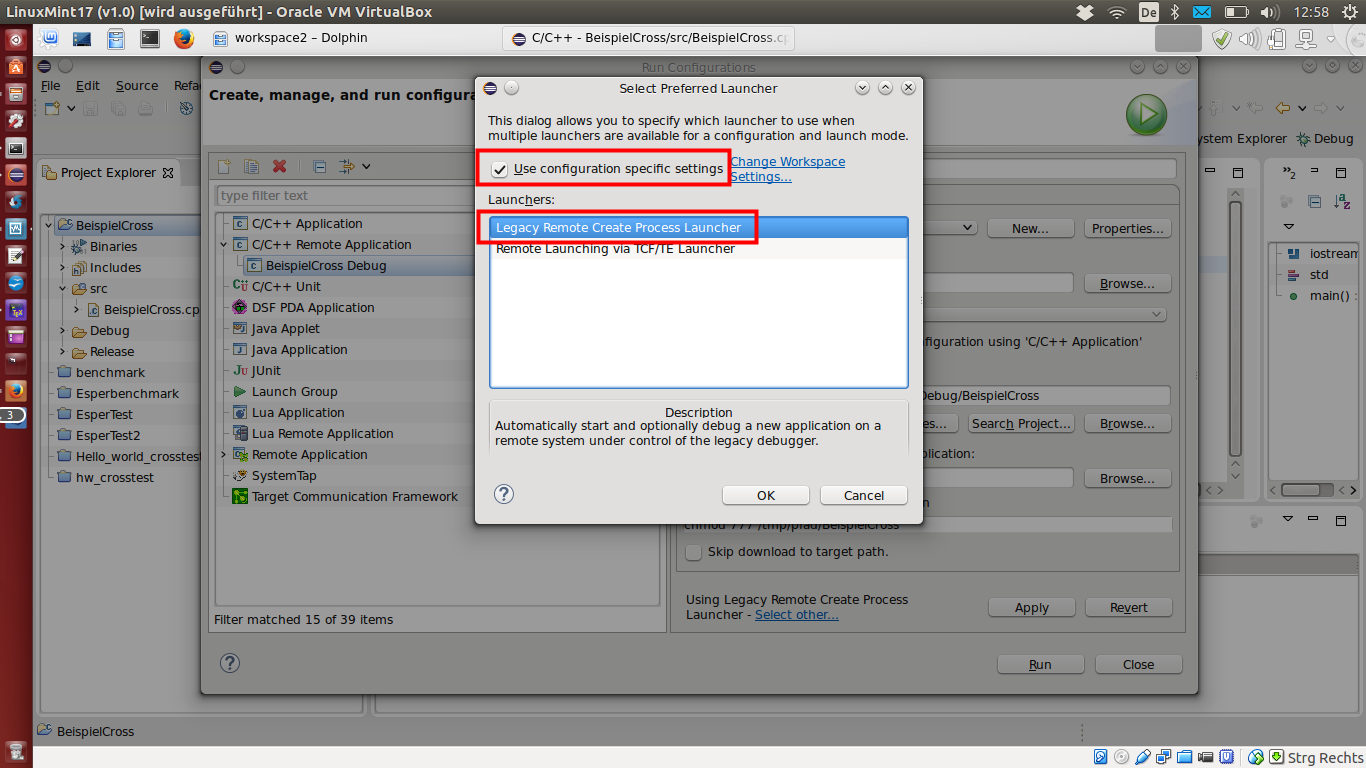
\includegraphics[width=0.9\linewidth]{./pictures/runf2.png}
%\caption[runf2]{}
%\label{fig:runf2}
%\end{figure}
%\begin{description}
%\item [P4:] Lässt sich die \textbf{Datei nicht ausführen} wurde das Programm ggf. nicht mit dem \glqq richtigen \textbf{Toolchain} \grqq kompiliert. In diese Fall sollte die Datei überprüft werden: 
%\end{description}
%\begin{figure}[h!]
%\centering
%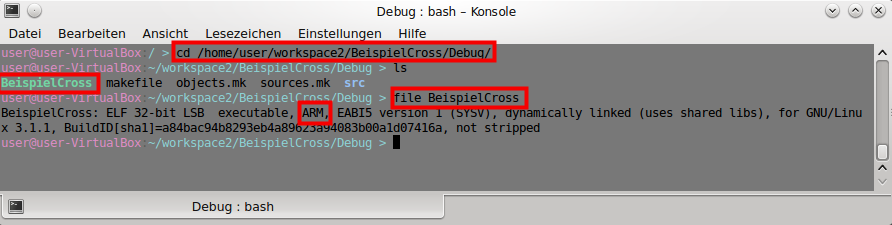
\includegraphics[width=0.9\linewidth]{./pictures/file.png}
%\caption[file]{Funktion der Threadgruppe}
%\label{fig:ThreadGroup}
%\end{figure}
% \vspace{5cm}
%Sollten der Parameter \glqq \textbf{ARM} \grqq nicht vorhanden sein, müssen die Einstellungen im Eclipse/vom Projekt überprüft werden. Hierbei hilft das Skript von Herrn \glqq Prof. Dr. Elmar Cochlovius\grqq. 
%
%
%\chapter{Remote Debug}
%Projekt remote Debuggen: \glqq \textbf{ Rechtsklick auf das Projekt } \grqq --> \glqq \textbf{Degbug As} \grqq --> \glqq \textbf{Debug Configurations ...} \grqq
%\begin{figure}[h!]
%\centering
%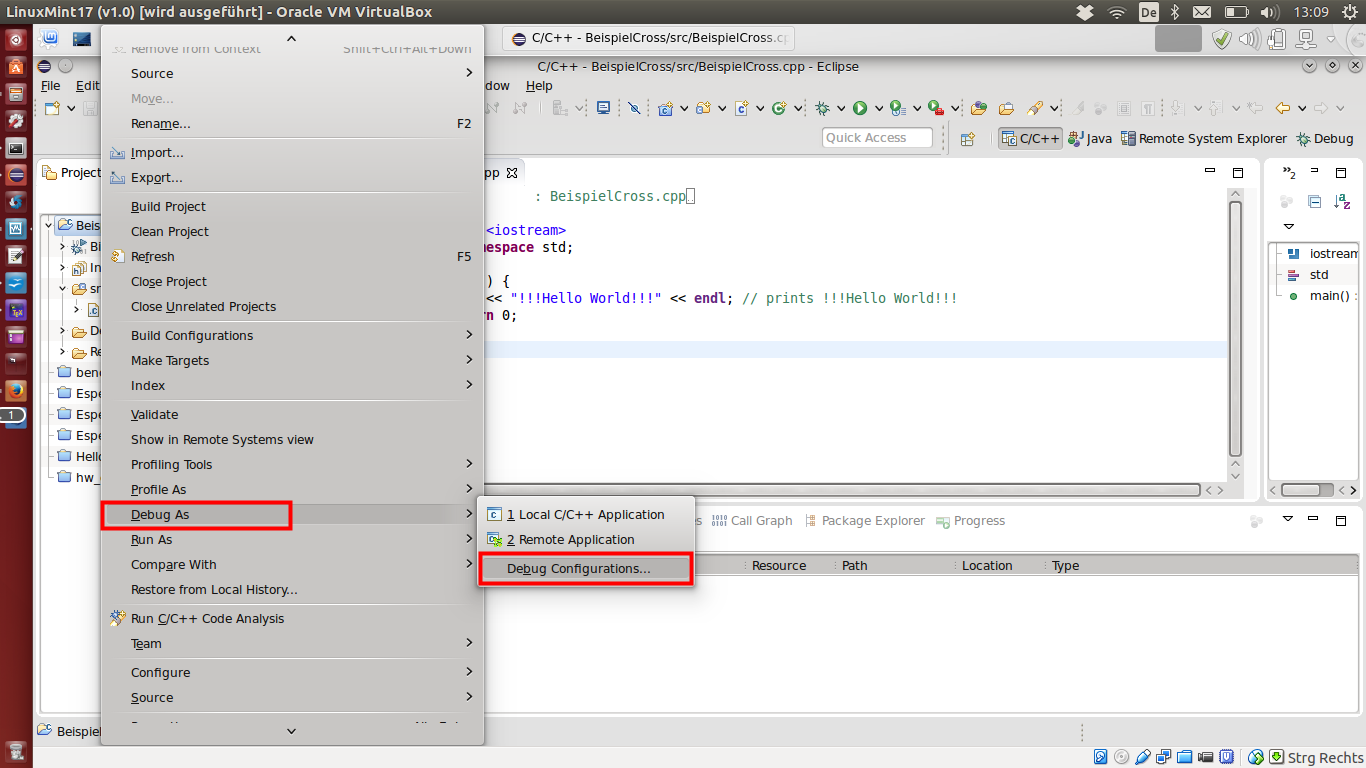
\includegraphics[width=0.9\linewidth]{./pictures/debug1.png}
%\caption[debug1]{}
%\label{fig:debug1}
%\end{figure}
%\newline
%In den dem sich öffnenden Fenster das bereits angelegte Projekt  wählen. Die rot markierten Felder sollten bereits konfiguriert sein. (siehe \glqq Cross Remote Compile  \grqq). 
%\begin{figure}[h!]
%\centering
%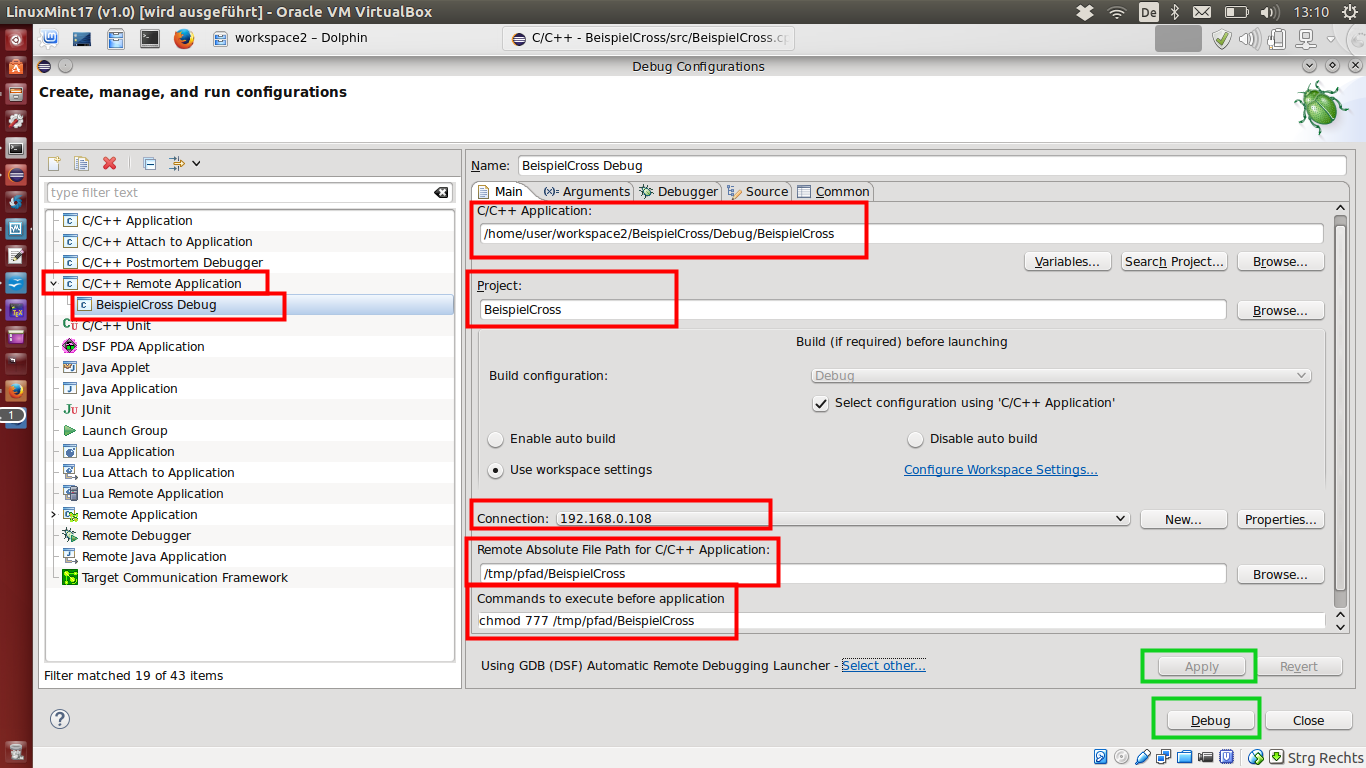
\includegraphics[width=0.9\linewidth]{./pictures/debug2.png}
%\caption[debug2]{}
%\label{fig:debug2}
%\end{figure}
%\newline
%Nun den Reiter \glqq \textbf{Debugger} \grqq öffnen:\\
%Hier muss das \glqq Präfix \textbf{GDB debugger} \grqq überschrieben werden, durch (rote Markierung): \textbf{arm-linux-gnueabihf-} 
%Außerdem ist es empfehlenswert die grün \glqq markierten \grqq Felder \glqq  anzuhacken \grqq
%(Optionen im Reiter \glqq Debugger \grqq \textbf{nicht vorhanden}): \grqq Fehlerbehandlung P1; \grqq 
%\begin{figure}[h!]
%\centering
%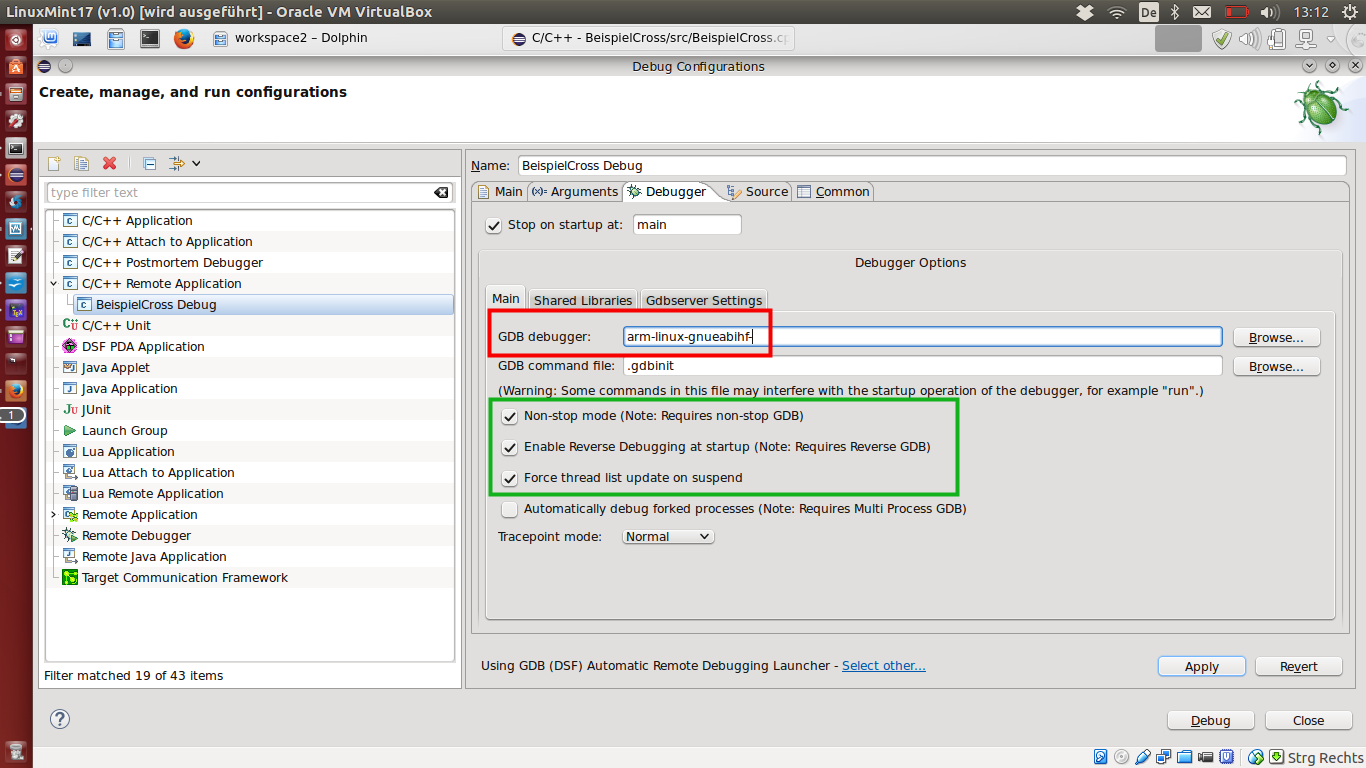
\includegraphics[width=0.9\linewidth]{./pictures/debug4.png}
%\caption[debug4]{}
%\label{fig:debug4}
%\end{figure}
%\newline
%Anschließend kann das Programm über die Button \glqq \textbf{Applay} \grqq und \glqq \textbf{Debugg} \grqq (grün maskiert)auf dem Target debuggt werden. Hierzu wird das Projekt auf dem lokalen  Gerät neu kompiliert, eine ausführbare Datei erzeugt und diese auf das Target neu übertragen. Diese übertragene, ausführbare Datei wird auf dem Target im Debugging-Modus gestartet. Sollte es zu Fehlern kommen: Siehe \grqq Fehlerbehandlung P2\grqq und \grqq Fehlerbehandlung P4\grqq
%\\
%GGf. erscheint ein Fenster, in welchem die Login-Daten eines Users des Target eingegeben werden müssen
%\begin{figure}[h!]
%\centering
%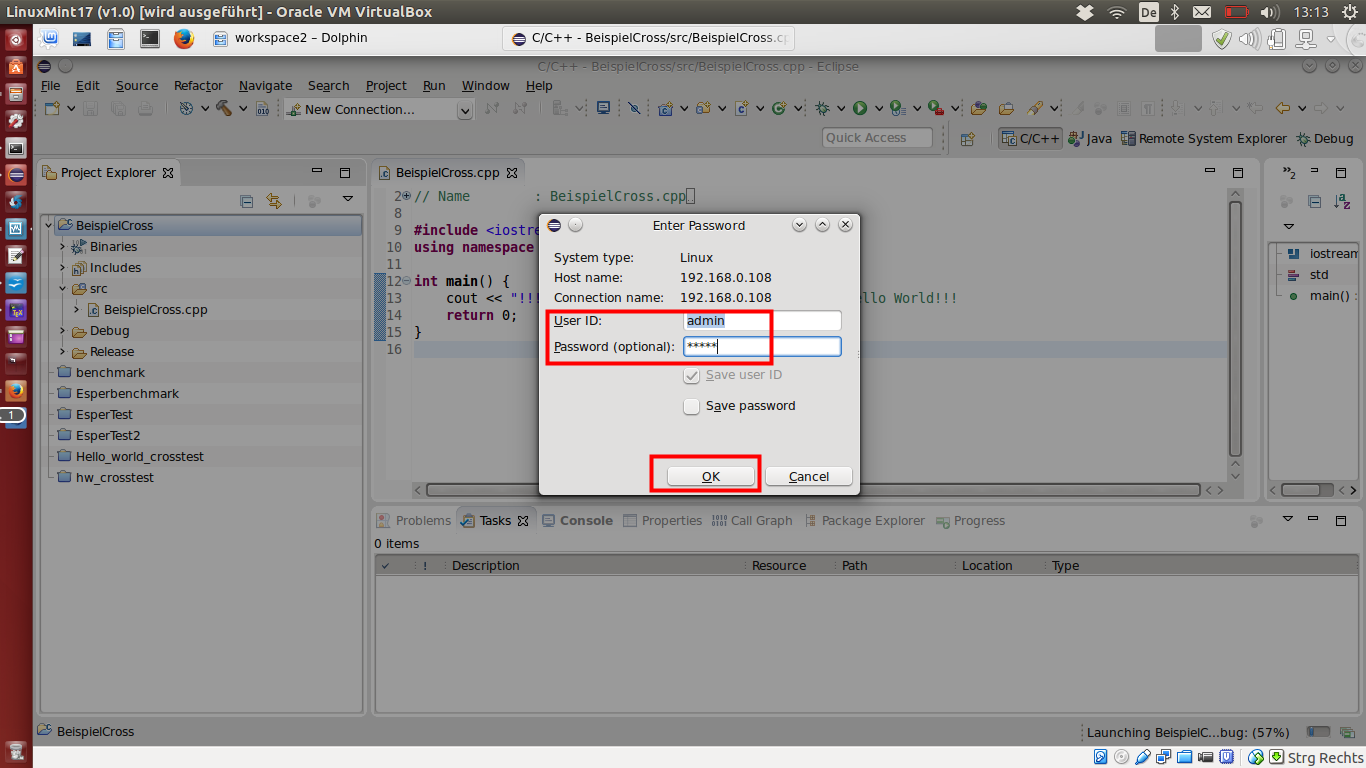
\includegraphics[width=0.9\linewidth]{./pictures/connect.png}
%\caption[connect]{}
%\label{fig:connect}
%\end{figure}
%\vspace{5cm}
%
%\section{Bekannte Fehler}
%\begin{description}
%\item [P1:] Der \glqq \textbf{Remote Debugger Process Launcher} \grqq muss über den \glqq \textbf{Select other ...} \grqq Link geändert werden.
%\end{description}
%\begin{figure}[h!]
%\centering
%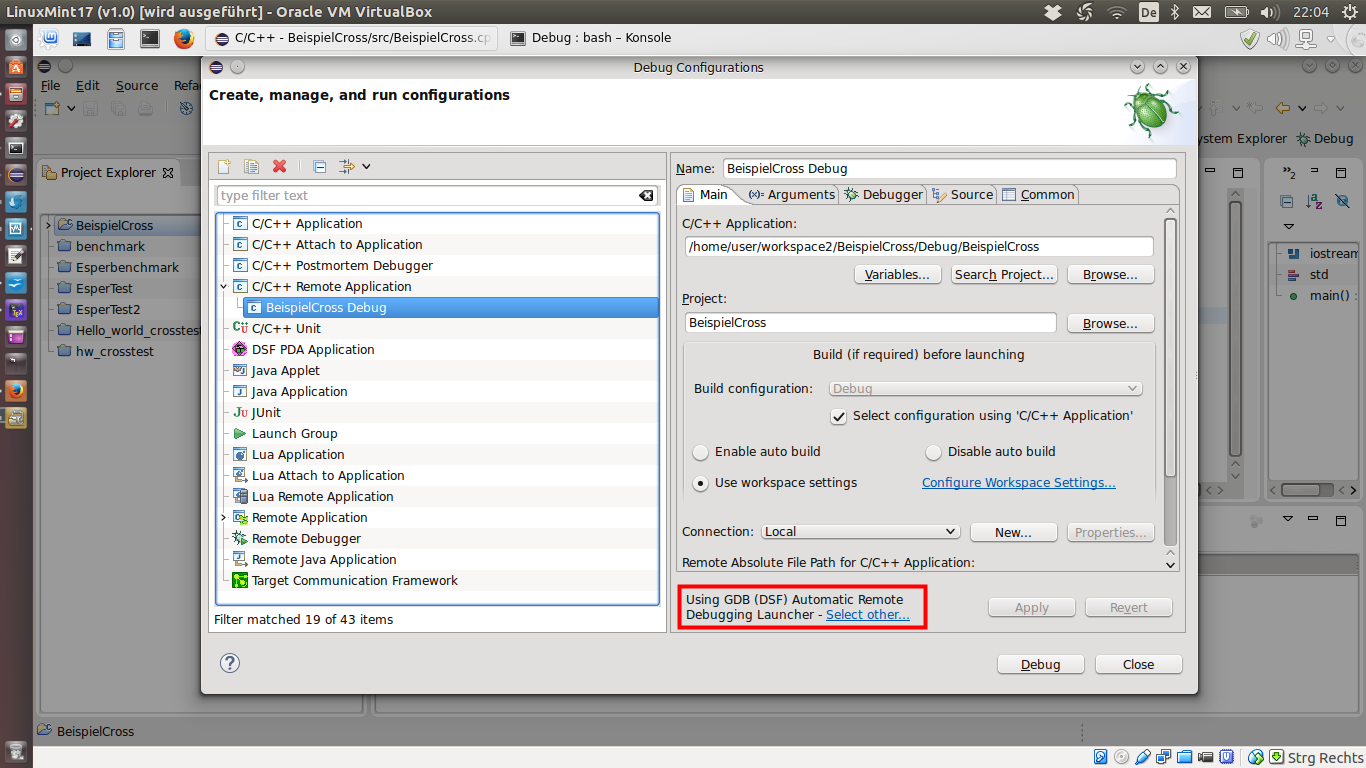
\includegraphics[width=0.9\linewidth]{./pictures/debugf1.png}
%\caption[debugf1]{}
%\label{fig:debugf1}
%\end{figure} 
%\vspace{1cm}
%In dem nachfolgenden Fenster \glqq \textbf{GDB(DSF) Automatic Remote Debugging Launcher} \grqq auswählen. Hierzu muss der \glqq  \textbf{Hacken} \grqq bei \glqq \textbf{Using configuration specific setings} \grqq gesetzt sein:
%\begin{figure}[h!]
%\centering
%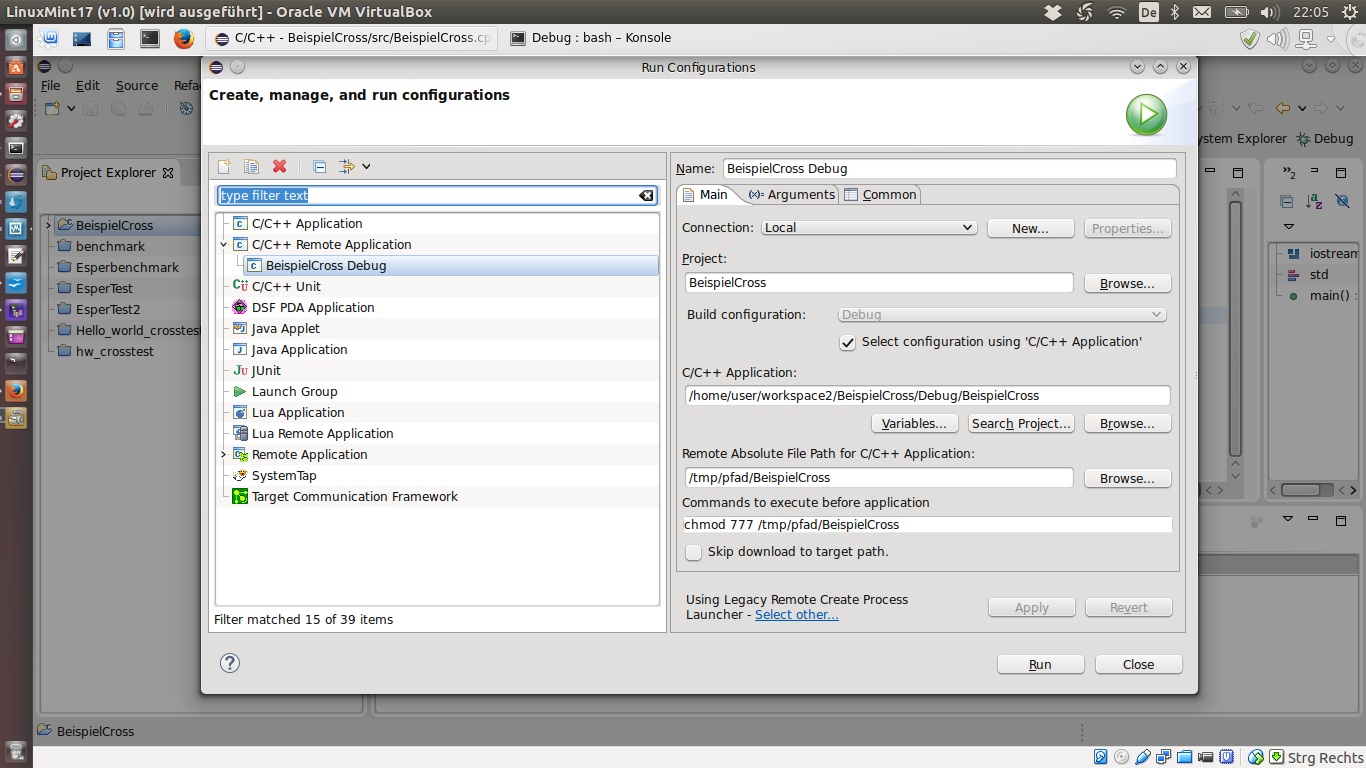
\includegraphics[width=0.9\linewidth]{./pictures/debugf2.png}
%\caption[debugf2]{}
%\label{fig:debugf2}
%\end{figure}
% \vspace{1cm}
%\begin{description}
%\item [P2:] Die \textbf{aktuelle Target IP} wurde unter \glqq \textbf{Remote System Explorer} \grqq nicht konfiguriert: Siehe Kapitel \glqq  \textbf{Netzwerkverbindung einrichten} \grqq. Oder die Geräte befinden sich nicht im \textbf{selben \glqq Subnetzwerk \grqq}
%\item [P4:] Lässt sich die \textbf{Datei nicht ausführen} wurde das Programm ggf. nicht mit dem \glqq richtigen \textbf{Toolchain} \grqq kompiliert. In diese Fall sollte die Datei überprüft werden: 
%\end{description}
%\begin{figure}[h!]
%\centering
%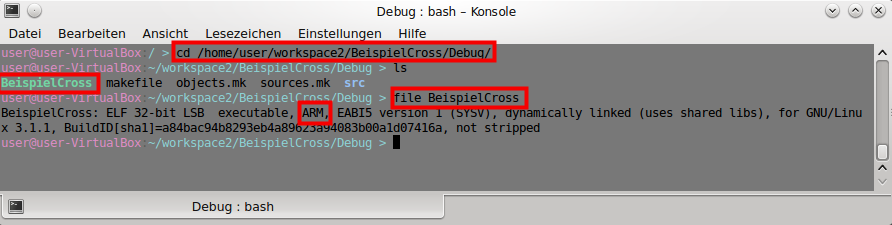
\includegraphics[width=0.9\linewidth]{./pictures/file.png}
%\caption[file]{Funktion der Threadgruppe}
%\label{fig:ThreadGroup}
%\end{figure}
% \vspace{1cm}
%Sollten der Parameter \glqq \textbf{ARM} \grqq nicht vorhanden sein, müssen die Einstellungen im Eclipse/vom Projekt überprüft werden. Hierbei hilft das Skript von Herrn \glqq Prof. Dr. Elmar Cochlovius \grqq. 
%
